\documentclass[11pt,letterpaper]{article}
\usepackage{acl2013}
\usepackage{times}
\usepackage{latexsym}
\usepackage{amsmath}
\usepackage{amssymb}
\usepackage{amsthm}
\usepackage{enumerate,paralist,enumitem}
\usepackage{verbatim}
\usepackage{mathtools}



\usepackage{graphicx}
\usepackage{caption,subcaption}
\usepackage{algorithm}
\usepackage{algorithmic}

\DeclareMathOperator*{\argmax}{arg\,max}

%\usepackage{authordate1-4}
\usepackage{multirow}

\usepackage{color,soul}
\usepackage{transparent}
\usepackage[usenames,dvipsnames,svgnames,table]{xcolor}
\newcommand{\Note}[1]{}
\renewcommand{\Note}[1]{\hl{[#1]}}
\newcommand{\NoteSigned}[3]{{\sethlcolor{#2}\Note{#1: #3}}}
\newcommand{\RemoveFF}[1]{\NoteSigned{Remove (FF)}{Crimson}{#1}}
\newcommand{\NoteFF}[1]{\NoteSigned{FF}{LightBlue}{#1}}
\newcommand{\NoteJE}[1]{\NoteSigned{JE}{LightGreen}{#1}}

\newcommand{\empirical}[0]{\ensuremath{\tilde{p}}}
\newcommand{\Data}[0]{\ensuremath{\mathcal{D}}}

\setlength\titlebox{6.5cm}    % Expanding the titlebox


\title{A Virtual Manipulative for Learning Log-Linear Models}


\author{
	 Author 1\\
	    XYZ Company\\
	    111 Anywhere Street\\
	    Mytown, NY 10000, USA\\
	    {\tt author1@xyz.org}
	  \And
	  Author 2\\
	    XYZ Company\\
	    111 Anywhere Street\\
	    Mytown, NY 10000, USA\\
	    {\tt author1@xyz.org}
 }
  
\date{}

\begin{document}

\maketitle

\begin{abstract}
We present a virtual manipulative for regularized conditional log-linear models. 
\end{abstract}

\section{Introduction}\label{sec:intro}
Given a dataset \Data{} consisting of $N$ points $\{( x_i, y_i)\}_{i=1}^N$, define empirical distribution
\begin{equation}
\empirical\left(y\ \mid\ x\right) = \frac{c(x,y)}{c(x)},
\end{equation}
where $c(x,y)$ and $c(x)$ represent bigram and unigram counts, respectively.

except for reading of data files, purely client-side $\Rightarrow$ very easy to set-up;
open-source;
data input format makes it extensible;
individual lessons can be tailored (e.g., hide/show buttons, different tool-tips for lessons)

Why do we focus on shapes, rather than words? \NoteFF{maybe we can argue via virtual manipulatives}

\NoteFF{what is the history of virtual manipulatives in teaching CS? NLP?} the HMM spreadsheet \cite{eisner-2002-tnlp}

\subsection{Regularized Conditional Log-Linear Models} \label{sec:model} 
Our aim is to provide an intuitive understanding of regularized conditional log-linear models. Given $\Data{} = \{( x_i, y_i)\ \mid\ 1 \le i \le N\}$ and $K$ features $f_k$ defined over \Data{} , we are interested in dissecting distributions 
\begin{equation}
\hat{p}_{\vec{\theta}}\left(y\ \mid\ x\right) = \frac{u(x, y)}{\sum_{y'} u(x,y')},
\label{eqn:conditional_loglin}
\end{equation}
where $u(x,y)$ represents the unnormalized probability
\begin{eqnarray}
u(x,y) & = & \exp{\left(\vec{\theta}\cdot \vec{f}(x,y)\right)}\\
& = & \exp{\left(\sum_{k=1}^K \theta_k f_k(x,y)\right)}.
\end{eqnarray}
As our model $\hat{p}_{\vec{\theta}}$ is fully described by the feature weights $\vec{\theta}$, we find the weights $\vec{\theta^*}$ that maximize the regularized conditional log-likelihood \eqref{eqn:reg_ll}:
\begin{equation}
F\left(\vec{\theta}\right) = \sum_{i=1}^N \log{\hat{p}_{\vec{\theta}}\left(y_i\ \mid\ x_i\right)} - C \cdot R\left(\vec{\theta}\right).
\label{eqn:reg_ll}
\end{equation}
Equivalently, we find $\vec{\theta^*}$ that solves equation \eqref{eqn:grad}:
\begin{equation}
\begin{aligned}
%\begin{split}
\nabla_{\vec{\theta}} F
 = &
\mathbb{E}_{\empirical{}}\left[\vec{f}(x,y)\right] 
- \mathbb{E}_{{\hat{p}_{\vec{\theta}}}}\left[\vec{f}(x,y)\right]\\
 & - C \nabla_{\vec{\theta}}R(\vec{\theta})\\
 = & 0.
%\end{split}
\end{aligned}
\label{eqn:grad}
\end{equation}
Here, $C \ge 0$ is the regularization penalty for the regularizer $R(\vec{\theta})$. Regardless of what regularization is applied, we will generally refer to the \textbf{full model} as that of \eqref{eqn:conditional_loglin} with objective \eqref{eqn:reg_ll}.\footnote{We consider models where $R(\vec{\theta}) = \vec{0}$ (no regularization), $R(\vec{\theta}) = \|\vec\theta\|_1$, and $R(\vec{\theta}) = \|\vec{\theta}\|_2^2$. See Section \ref{sec:overview} for more on regularization.}

\NoteFF{Is it further worth detailing difficulties people may have in learning about maxent models?}
However, the full model may present too many subtleties to be grasped all at once: reasoning about changing a single, particular $\theta_k$ requires consideration of a number of other variables, such as all other feature weights, the domain and range of the feature function $f_k$, and the amount of data available, among others. Therefore, we also consider ``simplified'' globally normalized models $\hat{p}_{\vec{\theta}}\left(y\right)$. These context-nescient models allow students to focus initially on understanding some of the core underlying concepts of exponential models, such as feature interations and weight tradeoffs, before progressing to conditional models.

%%%%%%%%%%%%%%%%%%%%%%%%%%%%%%%%%%%
%%%%%%%%%%%%%%%%%%%%%%%%%%%%%%%%%%%
%%%%%%%%%%%%%%%%%%%%%%%%%%%%%%%%%%%

\section{Pedagogical Aims}\label{sec:aims}
While any attempt to teach log-linear models must tackle the concepts, issues and difficulties addressed in the previous section, we found that enumerating specific pedagogical goals and expected take-aways helped focus the design of the virtual manipulative and the creation of individual lessons (c.f., Sections \ref{sec:overview} and \ref{sec:lessons}, respectively).
\subsection{Modeling Implications}
\begin{enumerate}
\item Choosing an appropriate model \textit{family}% (as in lesson 18, conditional, sequence, logistic regression)
\item Feature Design consideration:
\begin{itemize}
\item If the “striped” feature is predicted to occur less often than it actually does, you should raise its weight.
\item Frequent conditions more influential
\item binary vs. real valued features
\end{itemize}

\item Feature Interactions
\begin{itemize} 
\item Raising one weight may reduce or reverse the need to raise other weights.  This can be seen by watching the gradient as we slide the slider.
\item Can share features across conditions and this helps regularizer even if likelihood is the same
\item Features that only fire on conditions have no effect on conditional distribution
\item Feature conjunctions: fewer vs. more features
\item Feature that everything/nothing has --- weights go to $\pm \infty$
\item Opposing features, e.g., solid vs striped, where there are only 2 options
\item The initial setting where all weights = 0 gives the uniform distribution.
\begin{itemize}
\item Some further understanding of the entropy view?  (See below.)
\end{itemize}
\end{itemize}
\end{enumerate}

\subsection{Parameter estimation}
\begin{enumerate}[resume]
\item Some distributions can't be matched --- but you get generalization
\item It's possible to overfit the training data.  Regularization compensates for that and can in fact make you underfit.
\item bias vs. variance
\begin{itemize}
\item In particular, weights may zoom off to +infinity or -infinity if a feature is always or never present on the *observed* examples (may need to cook special datasets for this)
Gradient ascent and adaptive stepsize
\end{itemize}
\end{enumerate}

\subsection{Evaluating the Model, and Choosing an Appropriate Objective}
\begin{enumerate}[resume]
\item Likelihood always goes up if you follow gradient
\begin{itemize}
\item gradient = observed - expected count (- regularizer)

see eq \eqref{eqn:grad}
\item This is evident in the LL-bar at the top
\item Changes in gradient reflect portions of feature interactions (how minimizing the isolated $|\frac{\partial}{\partial \theta_k} F|$ might negatively affect some other partial $\frac{\partial}{\partial \theta_{k'}}F$.
\end{itemize}
\item importance of convexity: That is, we'll always find a unique $\vec{\theta^*}$ that solves \eqref{eqn:reg_ll}.
\item LL is maximized when you match the empirical (except for overfitting?)
\item matching vs. log-likelihood
Overfitting to a small training sample
Regularization (reduces the variance of your estimated parameters on a small training sample)
Smoothing = fitting the data imperfectly
(because the model has fewer parameters than outcomes, or because using too many parameters would be penalized by the regularizer)
Backoff smoothing = making use of backoff features and not just fine-grained features
(to avoid being penalized by the regularizer)
\end{enumerate}

We should note that we are \textit{not} concerned with computational issues here, e.g., that of tractably computing the normalization factors $Z(x_i)$. While efficiently computing the normalization factor is a crucial component to practical log-linear models, our primary concern is to provide a virtual manipulative that imparts a near-physical, intuitive understanding of log-linear models. 

\section{Virtual Manipulative Overview}\label{sec:overview}
See Figure \ref{fig:lesson1} for a screenshot.
\subsection{User Interface}
\begin{figure*}[t]
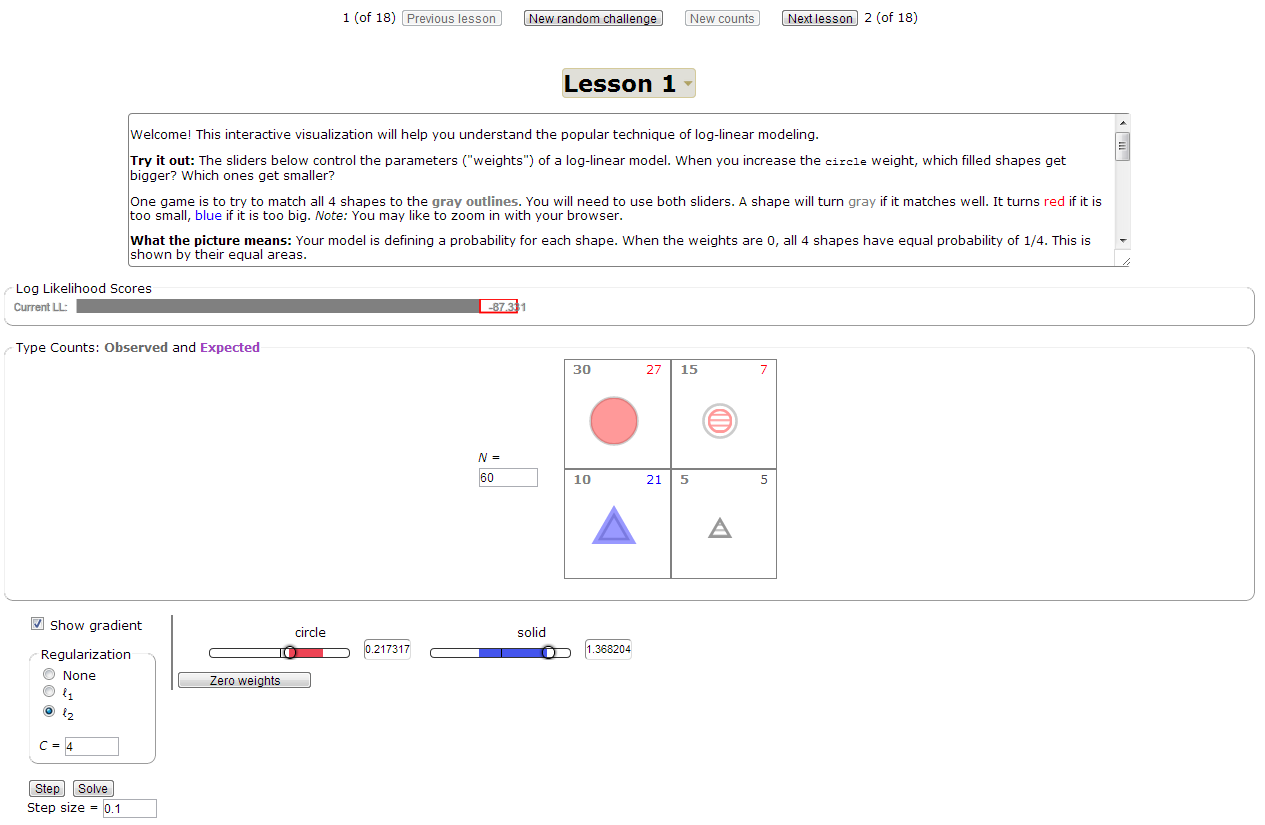
\includegraphics[scale=.5]{images/lesson1-grad-moved-nonewcounts-ell2-c4.PNG}
\caption{Screenshot of the first lesson from the virtual manipulative.}
\label{fig:lesson1}
\end{figure*}

\begin{figure}[t]
\begin{center}
\begin{subfigure}[b]{\columnwidth}
\centering
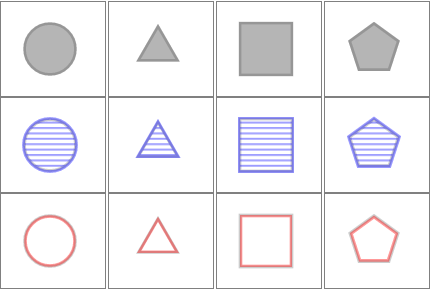
\includegraphics[scale=.5]{images/different_shapes_fills3x4.PNG}
\caption{Inventory of available shapes and fills. Note that while normally the color is indicative of the sign of \eqref{eqn:grad}, here the colors are solely provided as example.}
\label{fig:shape_inventory}
\end{subfigure}

\vspace{1em}
\begin{subfigure}[b]{\columnwidth}
\centering
\begin{tabular}{cccc}
\multirow{2}{*}{$\nabla_{\vec{\theta}}F(\vec{\theta}) $} & $<0$ & $= 0$ & $> 0$\\
& 
{\color{red}
\texttransparent{.5}{ red }
}
&
{\color{gray}
\texttransparent{.5}{ gray }
}
& 
{\color{blue}
\texttransparent{.5}{ blue }
}
\end{tabular}

\caption{How colors indicate the sign of \eqref{eqn:grad}.}
\label{fig:color_inventory}
\end{subfigure}

\vspace{1em}
\begin{subfigure}[b]{\columnwidth}
\centering
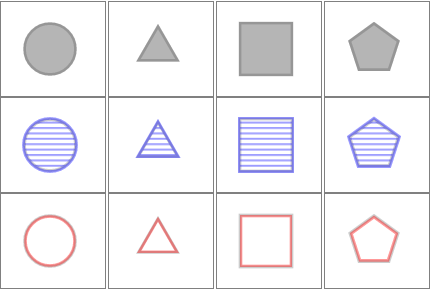
\includegraphics[scale=.5]{images/different_shapes_fills3x4.PNG}
\caption{\NoteFF{Replace with actual example text and images} Inventory of available shapes, fills, colors and other possible images. Note that while normally the color is indicative of the sign of \eqref{eqn:grad}, here the colors are solely provided as example.}
\label{fig:imgtxt_inventory}
\end{subfigure}
\end{center}
\end{figure}

The importance of color: what red vs. blue vs. gray means. This is in contrast to the importance of size

How does the user know how ``good'' the current parameter settings are? 

\subsubsection{Usability}
\begin{description}
\item[``New random challenge'']
\item[``New Counts'' button] The other use is to help the user experiment with datasets of different sizes, by changing N to scale the counts and then clicking "New counts."
\item[``Show gradient'']
\item[``Step'' and ``Solve'']
\item[``Peek at true'']
\item[Regularization] We consider models where $R(\vec{\theta}) = \vec{0}$ (no regularization), $R(\vec{\theta}) = \|\vec\theta\|_1$, and $R(\vec{\theta}) = \|\vec{\theta}\|_2^2$: we special-case the optimizer to handle the non-differentiable $\ell_1$ regularization, thus providing a friendly educational environment in which the student may explore the differences between $\ell_1$ and $\ell_2$ regularization.
\end{description}

\subsection{The Instructor Interface: Creating and Tailoring Lessons}
\subsubsection{Available Visualizations}
available shapes: four regular shapes: circle, square, triangle, pentagon; text; images (.jpg, .png)

shading: solid, striped, hollow


\subsubsection{Data description}
\begin{description}
\item[Required]

\begin{itemize}
\item a set of contexts (if missing, will be assumed to contain only one context)
\item a set of features; some of these may be marked as hidden
\item for each context, a set of events and visual positions for them \NoteFF{explain why this visual positioning is pedagogically important, i.e., aligning \texttt{circles} vs. \texttt{triangles}, and \texttt{solid} vs. \texttt{striped} can make feature contrasts stand out more}
\end{itemize}

\item[Optional]

\begin{itemize}
\item weights for some or all features (if missing, will be imputed from the prior N(0,I) and the supplied count vectors)
If no counts are supplied, then imputation is equivalent to simple sampling from N(0,I).
More generally, imputation requires MH sampling of the feature weights (and it’s wise to initialize the sampler to a MAP estimate found by the solver).  We may not implement this case immediately, in which case the weights may stay unknown.  In that case we have to gray out a couple of buttons and treat contexts without count vectors as if they had no observations.
\end{itemize}

%\item[Not done] \NoteFF{sadly, these didn't get tended to}
%\begin{itemize}
%\item 
%for each context, a total count $N_x$ (if missing, will be imputed from an integerized gamma prior and the supplied event counts and the weights)
%In practice, we can forbid the lesson-maker from supplying only some of the event counts in a given context.  In that case, either the whole count vector is given and $N_x$ is just the sum, or none of the count vector is given and $N_x$ is sampled from the gamma.
%for each (context, event) pair, a count (any missing counts for this context will be imputed)
%In practice, we can forbid the lesson-maker from supplying only some of the event counts in a given context.  In that case, if any of this count vector is missing, then the whole thing is missing, and we can impute it simply by sampling $N_x$ events from the distribution defined by the model weights.
%\end{itemize}
\end{description}

\subsection{The Back-End}
talk a bit about {\tt d3}, {\tt jQuery} and the various libraries/plugins used... nothing major, but it'll be good to outline here what exactly I used: jquery (1.7.2); jquery plugins tools, qtip, and ui

mention that some ui considerations can result in very slight rounding errors

solver: gradient ascent is simple (except for $\ell_1$ regularization), but it can take some finessing to make it visually appealing. We recursively call the solve function on a polynomial-decreasing schedule

\section{Provided Lessons}\label{sec:lessons}
\subsection{Joint Models}
\begin{enumerate}
\item 
4 types: rows %%$\{triangle, circle\} X columns \{solid, striped\}$
sliders only for circle and for striped
matchable

Questions: Lead students through navigation, ask simple understanding questions. If you make striped \& circle really big, what happens to the four probabilities?  First ignore the gray outlines.  What are the probabilities and expected counts (given N) when all features are 0?  If the total score of one object is 1 or 2 more than the total score of another object, what happens to their relative probabilities?  (for example, set circle to 1 and striped to 1.  What are the relative probabilities of the 4 objects?)  What happens to the probabilities when circle goes to +infinity?  to -infinity?  What happens to the log likelihood in these cases and why?  Now try to match the gray outlines, which represent the counts you’re trying to match.  If circles overall have too low a count, you should increase circle slider: the tooltip on the slider adds up the expected and observed counts for you.  Show them the “new random challenge button.”  Encourage them to check out the tooltips.
\item same as lesson 1 but sliders for triangle, circle, solid, striped
Questions: What’s the difference between increasing triangle and decreasing circle?  What if you increase triangle and circle by the same amount?  Does it help at all to have 4 sliders, or could you do just as well with 2 of them? Which 2?
\item same as lesson 2 but unmatchable (“XOR problem”)
Questions: Why can’t you match the probabilities of the 4 events? This also might be a good point to ask them to work through the details of computing Z, and the individual probabilities as fractions of Z. But can you still use your four sliders to match the aggregate expected counts of the two features?  Is it enough to use just two of the sliders and leave the others at 0?  What kind of inductive bias does the model have -- i.e., how are the the probabilities being smoothed when you match those counts?    
Log-likelihood game. Try to predict the data "as well as you can." Slide the sliders and watch the horizontal gray bar, which gives the log-likelihood—an overall measure of how well your model predicts the training data. How long can you you make the bar? How well do the shapes then match?

Matching game. Even if you can't match all 4 probabilities with your sliders, maybe you can match the 4 features. That is, try to make your model predict that among 60 shape tokens, there would be
\item same as lesson 3, but add a single conjoined feature so it’s matchable again Questions: Does it matter which conjoined feature is added?  Would it be ok to get rid of triangle and solid as in lesson 1?
\item rows {triangle, square, pentagon} x columns {solid, striped}
No features for specific shapes, but have a non-binary feature for number of sides: fires 3 times on triangle, 4 on square, 5 on pentagon.  Increasing this feature’s weight blows up pentagon at expense of triangle and perhaps expense of square.  Also have features for solid and for striped.
Question: what happens if you make the feature weight negative?  What would be different if if the feature were redefined from \# of sides to \# of sides - 3, or \# sides - 4?  If you added a pentagon feature, what would that allow you to do?

If this feature's weight is set to 1 (or -1), then what is the ratio of probabilities among the solid triangle, solid square, and solid pentagon? Try it! How does your answer change as you vary the weight of the solid feature?
\item rows {triangle, circle, square} X columns {solid, striped, hollow}
Questions: Is it hard to match by hand?  Learn about gradient display.
Understanding the hints. Recall the two games from lesson 3. The hint on the slider can be interpreted as a hint for either game.

Log-likelihood game. Following the hint on the circle slider will increase the log-likelihood. That's because the length of the hint bar is the partial derivative of the log-likelihood with respect to the circle weight.

Matching game. Following the same hint will also improve the match between the expected and observed number of circles. That's because the length of the hint bar is (observed circles - expected circles).


Extra fun. If you enjoy trying to match the gray outlines, you can get more puzzles of this kind. Clicking "New random challenge" (at the top of the page) picks a new log-linear distribution and samples N observed events from it. Your job as a statistician is to use those N events (the gray counts and gray outlines) as clues to help you guess the true distribution. You can do a good job by playing the games above to maximize log-likelihood. Then click "Peek!" to reveal the true parameters and how well they would do on log-likelihood. (But remember lesson 2, and don't be disappointed if you found different parameters that define exactly the same distribution.)

Warning: Reducing N before you generate the new challenge will give you fewer clues—making your statistical task harder! Your random sample of N events will be sparse and perhaps idiosyncratic. In fact, you can see the variance among random samples by clicking "New counts" to see another sample you could have gotten—with different observed counts indicated by the different-sized gray outlines. So if you try too hard to match them, you might be overfitting the training data (achieving an even better training log-likelihood than the true parameters would) rather than finding the true parameters. More about that soon ...
\item %lesson 7
Like lesson 6, but now unmatchable (maybe because the true model has some extra features not shown).  
Question: Learn about solver and gradient ascent. Introduced to step size box, step button and solve button.  What solution does the model find?
``However, there will still be red and blue left on some of the shapes. How well do the expected counts for individual kinds of circles match the training data? Why?'' (actually, answer for triangles: expected = observed = 195)
\item %lesson 8
Like lesson 7, and now the solver overfits because all of the squares have count 0: so the weight goes to -infinity and we estimate the probabilities of the squares as 0, which is not good for a smoothing method.  Learn about regularization.  Question: What effect does regularization have on the expected counts of the stripes?  How about the expected counts of the others?  On the log-likelihood? why? How is this related to smoothing?  
students are encouraged to retry previous lessons to ease into regularizaiton on simpler models
\item %lesson 9 
Like lesson 7, but this time get overfitting by reducing N.  Here the student should generate a number of random challenges with different values of N, and use the solver.  Question: For a given amount of regularization, is there more smoothing of the probabilities with high N or with low N?  (Distinguish between the counts and the probabilities here.)  For a given N, is there more smoothing with high or low $sigma^2$?
What if you use ℓ1 regularization instead? Also, in this case, did any of your weights come out to exactly 0? (This is often the case for the optimal solution under ℓ1.)

Smoothing on larger data. Regularization had a strong smoothing effect on this small dataset. However, what if you had more evidence? You can scale up the counts by increasing N in the text box to the left of the shapes. Open a second window so that you can easily compare N = 50 with N = 5000. In both cases, solve with ℓ2 regularization with C = 1.

What happens to the optimal log-likelihood and why?
What happens to the weights and why?
The observed counts increased by a factor of 100. Which of the expected counts increased by a factor of much less than 100?
The model has decreased its estimated probability for those outcomes. Which other outcomes did it move their probability to?
What happens if you also increase C by a factor of 100?
Discussion: tradeoff between N and C. Remember that the optimal θ maximizes F = (log-likelihood - regularizer), a difference of two functions.
Increasing N stretches the first function vertically, so that it has more influence on the shape of F. So the more training data there is, the more the solver just tries to fit the training data.

Increasing C stretches the second function vertically, so that it has more influence on the shape of F. So the stronger the regularizer is, the harder the solver will try to keep the weights close to 0.

Doubling both N and C will just stretch F vertically, leaving the optimal θ unchanged.
\item %lesson 10
like lesson 7, but now we have too many features: we have the 9 conjoined features like triangle\&solid, triangle\&striped, etc.  So each shape can now be manipulated independently.
Question:  Note that each event now has its own feature.  This makes it easy to manipulate the probabilities individually -- try it by hand and with the solver.  The probabilities should match exactly.  Analogously, here is a fairly easy math question: Suppose you have 9 letters a,b,...i where a has feature 1 (only), b has feature 2 (only), etc.  You would like to match the observed probabilities $p(a)=p_1, p(b)=p_2$, etc., where $p_1+...+p_9=1$.  How could you set $theta_1, theta_2$, etc. to achieve this?   Because you have enough parameters to match the training data exactly, you will need some regularization for smoothing.  What is the effect of regularization in this setting where events don’t share features at all? 
\end{enumerate}

\subsection{Conditional Models}
\begin{enumerate}[resume]
\item First conditional model: brief warmup for lesson 12 below, except make them all circles and label the rows that were formerly triangle, circle, square as English, Polish, Martian (and change the feature names accordingly).  This is formally identical to lesson 12.  So we are predicting fill color based on language.  Note that we have a larger corpus of English than of Polish, and no corpus of Martian (yet!).
\item Conditional model: like lesson 7 except we now condition on the row.  “We are now showing each language as a separate shape.  Or equivalently, imagine that you already had a shape, and the event is that someone came along and picked a pattern to fill it with.  We are no longer predicting probabilities of different shapes.”  The only sliders are for solid, striped, and hollow (this is a little simpler than lesson 7).  Drop the square row for simplicity -- no, on second thought, just make that row completely unobserved so that we see generalization.  Separate the rows into different panels.  The triangle counts are (70,20,10) while the circle counts are (5,5,5) and the square counts are (0,0,0).   Note that a separate N will be shown for each context (and changing that N will generate a new random challenge in that context).  Because we have no features that pay attention to context, it’s as if we were aggregating down the column.  
Questions: What happens to triangle fit when you match the circles by hand?  How about vice-versa?  Which has the better log-likelihood and why?  If you follow the gradients to maximize the likelihood, does that fit the triangles or the circles or somewhere in between?  [The circles counts should be high enough so that the answer is clearly “in between.”]   Do the squares (unobserved) then act more like the triangles or the circles?
\item Like lesson 12, but now we have only the solid triangle (with count 100) -- so there’s only one outcome for triangles.  (The others essentially have probabilities tied to 0.)  Now the parameters only affect circles, so it pays to match the circles.  Let’s remove the hollow square as well, just for fun.
This example shows one way that maximizing conditional likelihood is different from maximizing joint likelihood.

In the English (circle) context, it is now only possible to talk about solid. Since English is popular, this means there are lots of solid shapes in our training data. Yet what are the weights that maxmize the conditional log-likelihood? Discuss why this is.
\item Like lesson 12, but add sliders for the triangle, circle, and square features (in addition to the existing solid, striped, and hollow).  Question: Why don’t these new sliders do anything?
\item Like lesson 14, but add 3 sliders for conjoined features “solid circle,” “solid triangle,” “solid square.”  These are our first bigram features, whereas solid was our unigram feature.  Question: Demonstrate multiple solutions that give you the same likelihood.  (For example, run solver from different starting points.)  Which has the best regularization penalty?   (Turn on regularization and solve again.)  How about if we use l1 regularization?  What is the effect of that on smoothing?  How is this related to backoff?  [Note: Focus this on tuning solid circle / solid triangle / solid square versus just tuning solid.  Probably the data should be generated from a model where the backoff features like solid are indeed strong.  Also, make $sigma^2$ large so that the regularization penalty is easier to see.]
\item Logistic regression.  Contexts are the following phrases or objects being classified:
…
...
In each context we have a hollow circle for “no” and a solid circle for “yes”.  (Might be better to show as  - and +.)  The features are always features of the context conjoined with blue:
solid\&...
solid\&...
Maybe classify languages as Indo-European or agglutinative or something?  But classifying baby names as male vs. female is probably better.  The observed counts are the number of times that name has been observed attached to a boy vs. a girl.  Pick a small set of names to use as data.  We can have features for multisyllabic, \# of syllables (this is integer-valued), starts with a vowel, ends with a vowel, ends with -a, ends with -ja, and prevalence in sports (this is a real number in [0,1], perhaps the fraction of days that it appears in the sports section of the newspaper).  “Venus” might be misclassified.  Emphasize that many more features could be generated manually or automatically (link to nltk lesson).

Taking the "unigram"/"bigram" analogy more seriously, here is a "bigram language model" over a sequence of filled shape events. The choice of the next filled shape depends on what its predecessor was. The predecessor is the context.

We include the usual "unigram" features that consider only the event without its context. We have features for each of the 9 filled shape events, as well as "backed-off" unigram features for each of the 3 fill-patterns and each of the 3 shapes. A backoff feature such as circle fires on multiple events and thus can help capture generalizations across events, such as "circles are common" (analogous to "words ending in -ing are common").

How about the "bigram" features? We'll back off here by modeling just 3 general features that look at the event and the context together:

Is the event identical to the previous event?
Does the event have the same shape as the previous event?
Does the event have the same fill-pattern as the previous event?
\item Here's a little application of log-linear modeling to text categorization. Each natural-language phrase is classified as to whether it is spam.

Your job is to poke around and figure out what is going on here. Remember, we must be modeling some conditional probability distribution p(outcome | context).

What are the contexts? Why do most (but not all) contexts have count 1?
What are the possible outcomes? How are they displayed as shapes?
What kind of information below indicates that a particular training phrase has been labeled as spam?
Which are the two test phrases included below? How do you know?
If you train this model without regularization, what happens to the log-likelihood and the weights? Why?
If you train this model with regularization, how does it classify the two test phrases? Look at the weights: what features helped it make this classification?
You might think that 'fortune' fires on any phrase that contains the word 'fortune'. But lesson 14 suggests that can't quite work. Let's be precise: what (context,outcome) pairs is 'fortune' really defined to fire on?
mentions money is a binary feature. What are some words that cause it to fire? How did you find out?
Is the feature 'yada' a binary feature, or a counting feature? That is, does fyada return 1 or 3 on yada yada yada? How did you find out?
Which of the non-spam messages does your trained model think is spammiest? How do you know?
This is an example of binary classification, since there are just two possible decisions. How would you extend the approach to do three-way classification of a phrase as {spam,work,fun}?

\item %lesson 18
conclusion
\end{enumerate}

\bibliography{tnlp}
\bibliographystyle{acl}

\end{document}
